%Lecture 4
%Copyright (C) 2019  Patrick Diehl
%
%This program is free software: you can redistribute it and/or modify
%it under the terms of the GNU General Public License as published by
%the Free Software Foundation, either version 3 of the License, or
%(at your option) any later version.

%This program is distributed in the hope that it will be useful,
%but WITHOUT ANY WARRANTY; without even the implied warranty of
%MERCHANTABILITY or FITNESS FOR A PARTICULAR PURPOSE.  See the
%GNU General Public License for more details.

%You should have received a copy of the GNU General Public License
%along with this program.  If not, see <http://www.gnu.org/licenses/>.
\documentclass[12pt,t]{beamer}

\beamertemplatenavigationsymbolsempty

% usepackage
%\usepackage{template/dbt}
\usepackage{listings,graphics}

\definecolor{comments}{RGB}{81,81,81}
\definecolor{keywords}{RGB}{255,0,90}

% lstlisting
\lstset{
    language=C,
    basicstyle=\footnotesize\ttfamily,
    keywordstyle=\color{keywords},
    showspaces=false,
    showstringspaces=false,
    commentstyle=\color{blue}\emph
    %frame=single,
    %rulecolor=\color{comments},
    %rulesepcolor=\color{comments},
    %backgroundcolor = \color{lightgray}
}

\usetheme{default}

\usepackage[
    type={CC},
    modifier={by-nc-nd},
    version={4.0},
]{doclicense} 

\newcommand{\courseurl}[0]{https://www.cct.lsu.edu/\string~pdiehl/teaching/2021/4997/}
\newcommand{\coursetimeline}[0]{https://www.cct.lsu.edu/~pdiehl/teaching/2021/4997/timeline.pdf}
\newcommand{\coursesyllabus}[0]{https://www.cct.lsu.edu/~pdiehl/teaching/2021/4997/syllabus.pdf}
\newcommand{\coursename}[0]{Math 4997-3}
\newcommand{\coursemailinglist}[0]{https://mail.cct.lsu.edu/mailman/listinfo/par4997}
\newcommand{\coursesemester}{Fall 2021}








% frame slide
\title{\coursename}
\subtitle{Lecture 4: N-Body simulations, Structs, Classes, and generic functions}

%\author{\href{}{}}
%\institute {
%    \href{}{\tt \scriptsize \today}
%}
\date {
 \tiny \url{\courseurl}
\vspace{2cm}
\doclicenseThis  
  
}



\usepackage{ifxetex}
\usepackage{tikz}

\ifxetex
\usepackage{fontspec}
\setmainfont{Raleway}
\fi

\ifluatex
\usepackage{fontspec}
\setmainfont{Raleway}
\fi

\begin{document} {
    \setbeamertemplate{footline}{}
    \frame {
        \titlepage
    }
}

\frame{

\tableofcontents

}

\AtBeginSection[]{
  \begin{frame}
  \vfill
  \centering
  \begin{beamercolorbox}[sep=8pt,center,shadow=true,rounded=true]{title}
    \usebeamerfont{title}\insertsectionhead\par%
  \end{beamercolorbox}
  \vfill
  \end{frame}
}

%%%%%%%%%%%%%%%%%%%%%%%%%%%%%%%%%%%%%%%%%%%%%%%%%%%%%%%%%%%%%%%%%%%%%%%%%%%%%%
\section{Reminder}
%%%%%%%%%%%%%%%%%%%%%%%%%%%%%%%%%%%%%%%%%%%%%%%%%%%%%%%%%%%%%%%%%%%%%%%%%%%%%%

\begin{frame}{Lecture 3}
\begin{block}{What you should know from last lecture}
\begin{itemize}
\item Iterators
\item Lists
\item Library algorithms
\item Numerical limits
\item Reading and Writing files
\end{itemize}
\end{block}
\end{frame}


%%%%%%%%%%%%%%%%%%%%%%%%%%%%%%%%%%%%%%%%%%%%%%%%%%%%%%%%%%%%%%%%%%%%%%%%%%%%%%
\section{$N$-body simulations}
%%%%%%%%%%%%%%%%%%%%%%%%%%%%%%%%%%%%%%%%%%%%%%%%%%%%%%%%%%%%%%%%%%%%%%%%%%%%%%

\begin{frame}{$N$-body simulations\footnote{\tiny By Michael L. Umbricht - Own work, CC BY-SA 4.0}}

\begin{figure}
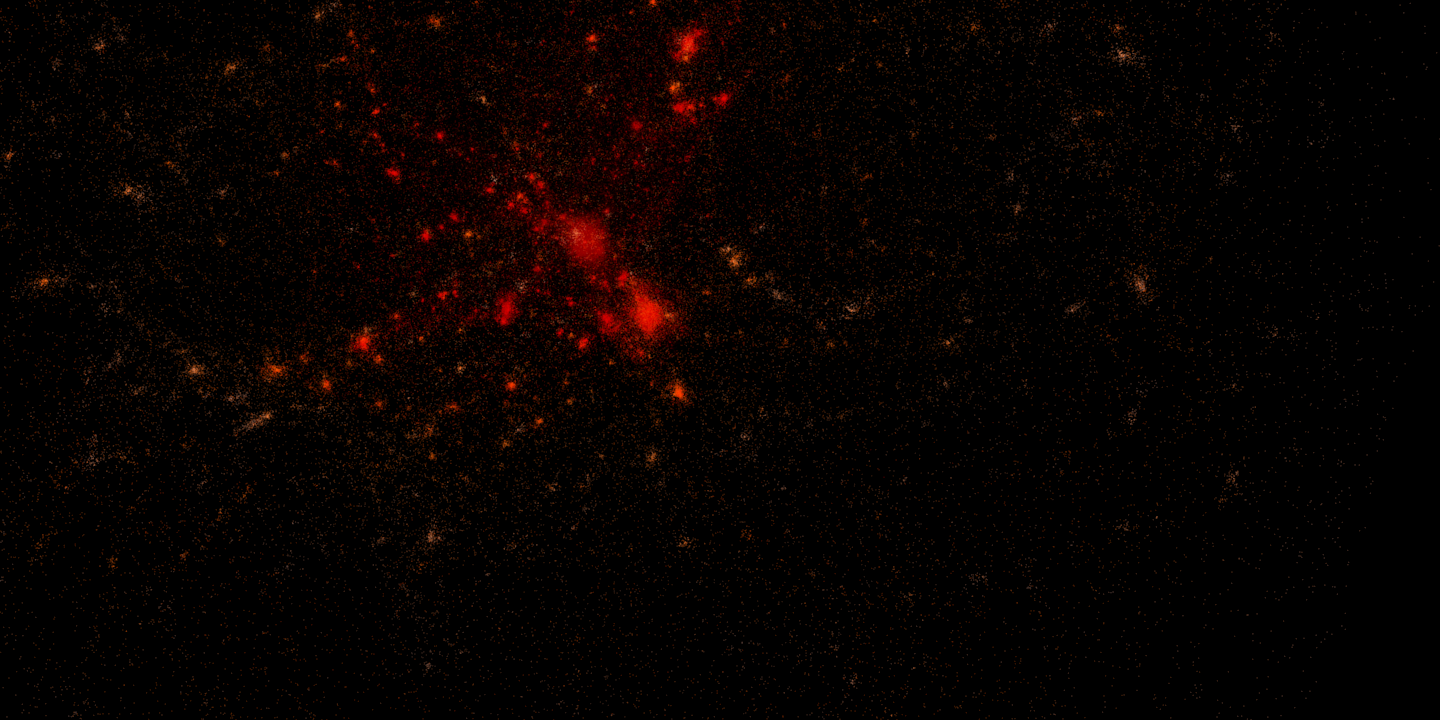
\includegraphics[width=0.5\linewidth]{./images/Galaxy_cluster_sim.png}
\end{figure}


The $N$-body problem is the physically problem of predicting the individual motions of a group of celestial objects interacting with each other gravitationally.

\begin{block}{Informal description:}
Predict the interactive forces and true orbital motions for all future times of a group of celestial bodies. We assume that we have their quasi-steady orbital properties, e.g.\ instantaneous position, velocity and time.
\end{block}

\end{frame}


\begin{frame}{Recall: Vectors and basic operations}


\begin{block}{Vectors}
\centering
$\mathbf{u}=(x,y,z)\in \mathbb{R}^3$\\
\begin{enumerate}
\item Norm: $\vert \mathbf{u} \vert = \sqrt{x^2+y^2+z^2}$
\item Direction: $\frac{\mathbf{u}}{\vert \mathbf{u}\vert}$
\end{enumerate}
\end{block}
\begin{block}{Inner product}
\centering
$\mathbf{u}_1 \circ \mathbf{u}_2 = x_1x_2 + y_1y_2 + z_1z_2 $
\end{block}
\begin{block}{Cross product}

\begin{center}
$\mathbf{u}_1 \times \mathbf{u}_2 = \vert\mathbf{u}_1 \vert \vert\mathbf{u}_2 \vert sin(\theta) \mathbf{n}  $
\end{center}
where $\mathbf{n}$ is the normal vector perpendicular to the plane containing $\mathbf{u}_1$ and $\mathbf{u}_2$.
\end{block}

\end{frame}

\begin{frame}{Stepping back: Two-body problem}
Let $m_i,m_j$ be the masses of two gravitational bodies at the positions $\mathbf{r}_i,\mathbf{r}_j\in\mathbb{R}^3$

\begin{block}{Three key laws:}
\begin{enumerate}
\item The Law of Gravitation: The force of $m_i$ acting on $m_j$ is \\
$\mathbf{F}_{ij}= G m_i m_j \frac{\mathbf{r}_j-\mathbf{i}_2}{\vert \mathbf{j}_1-\mathbf{r}_i \vert^3}$
\item The Calculus: 
\begin{enumerate}
\item The velocity of $m_i$ is $\mathbf{v}_i = \frac{d \mathbf{r}_i}{dt}$
\item The acceleration of $m_i$ is $\mathbf{a}_i \frac{d \mathbf{v}_i}{dt}$
\end{enumerate}
\item The second Law of Mechanics: \\
 $\mathbf{F}= m \mathbf{a}$ (Force is equal mass times acceleration)
\end{enumerate}
\end{block}
The universal constant of gravitation $G$ was estimated as $6.67408\cdot 10^{-11}m^3kg^{-1}s^{-2}$ in 2014~\cite{mohr2016codata}.
\end{frame}



\begin{frame}{Put all together: Equation of motion}
Derivation for the first body:
\begin{columns}
\begin{column}{0.5\textwidth}
\begin{align*}
\mathbf{F}_{ij}&=G m_i m_j \frac{\mathbf{r}_j-\mathbf{r}_i}{\vert \mathbf{r}_j-\mathbf{r}_i \vert^3}  \\
m_1 \mathbf{a}_i &= G m_i m_j \frac{\mathbf{r}_j-\mathbf{r}_i}{\vert \mathbf{r}_i-\mathbf{r}_j \vert^3} \\
\frac{d \mathbf{v}_i}{dt} & = G m_j \frac{\mathbf{r}_j-\mathbf{r}_i}{\vert \mathbf{r}_j-\mathbf{r}_i \vert^3} \\
\frac{d^2 \mathbf{r}_i}{dt^2} & = G m_j \frac{\mathbf{r}_j-\mathbf{r}_i}{\vert \mathbf{r}_j-\mathbf{r}_i \vert^3}
\end{align*}
\end{column}
\begin{column}{0.5\textwidth}  %%<--- here
    \begin{center}
    \begin{tikzpicture}
\draw (-2,0) circle (0.5cm);
\draw (2,0) circle (0.275cm);
\node at (-2,0) {$m_1$};
\node at (2,0) {$m_2$};
\draw[->] (-1.5,0)--(-1,0);
\draw[->] (1.7,0)--(1,0);
\node[below] at (-1,0) {$\mathbf{F}_1$};
\node[below] at (1,0) {$\mathbf{F}_2$};
\end{tikzpicture}
     \end{center}
\end{column}
\end{columns} 
\vspace{0.5cm}
For the second body follows:
$\frac{d^2 \mathbf{r}_2}{dt^2}  = G m_1 \frac{\mathbf{r}_1-\mathbf{r}_2}{\vert \mathbf{r}_1-\mathbf{r}_2 \vert^3}$ \\
\vspace{0.5cm}
Note that we used Newton's law of universal gravitation~\cite{newton1833philosophiae}.

\end{frame}

\begin{frame}{The $N$-body problem}

\begin{block}{The force for body $m_i$}
$\mathbf{F}_i = \sum\limits_{j=1,i\neq j}^n \mathbf{F}_{ij} = \sum\limits_{j=1,,i\neq j}^n G  m_j \frac{\mathbf{r}_j - \mathbf{r}_i}{\vert \mathbf{r}_j - \mathbf{r}_i\vert^3} $
\end{block}

\begin{block}{Law of Conservation:}
\begin{enumerate}
\item Linear Momentum: $\sum\limits_{i=1}^n m_i \mathbf{v}_i = M_0$
\item Center of Mass: $\sum\limits_{i=1}^n m_i \mathbf{r}_i = M_0 t + M_1$
\item Angular Momentum: $\sum\limits_{i=1}^n m_i (\mathbf{r}_i \times \mathbf{v}_i) = \mathbf{c}$
\item Energy: T-U=h with \\
$ T = \frac{1}{2} \sum\limits_{i=1}^n m_i \mathbf{v}_i \circ \mathbf{v}_i  , U= \sum\limits_{i=1}^n \sum\limits_{j=1}^n G \frac{m_i m_j}{\vert\mathbf{r}_i - \mathbf{r}_j\vert} $
\end{enumerate}
\end{block}
More details: Simulations~\cite{aarseth2003gravitational} and Astrophysics~\cite{aarseth2008cambridge}.
\end{frame}

\begin{frame}{Algorithm}

\begin{figure}
\begin{tikzpicture}
\draw (-3.75,0) rectangle (2,1) node[pos=.5] {Compute the forces};
\draw[->](-0.75,0) -- (-0.75,-1);
\draw (-3.75,-2) rectangle (2,-1) node[pos=.5] {Update the posotions};
\draw[->](-0.75,-2) -- (-0.75,-3);
\draw (-3.75,-4) rectangle (2,-3) node[pos=.5] {Collect statiscal information};
\draw[->] (2,-3.5) -- (3,-3.5) -- (3,0.5) -- (2,0.5);
\end{tikzpicture}
\end{figure}

\end{frame}

\begin{frame}[fragile]{Complexity of force computation}

\begin{block}{Force computation: Direct sum}
\begin{lstlisting}
for(size_t i = 0; i < bodies.size(); i++)
for(size_t j = 0; j < bodies.size(); j++)
//Compute forces
\end{lstlisting}
\end{block}

\begin{block}{Advantage:}
Robust, accurate, and completely general
\end{block}

\begin{block}{Disadvantage:}
\begin{enumerate}
\item Computational cost per body $\mathcal{O}(n)$ 
\item Computational cost for all bodies $\mathcal{O}(n^2)$ 
\end{enumerate}
\end{block}
Tree-based codes or the Barnes-Hut method~\cite{barnes1986hierarchical} reduce the computational costs to $\mathcal{O}(n\log(n))$. More details~\cite{knuth1997art}.
\end{frame}

\begin{frame}{Update of positions}
Assume we have computed the forces already, using the direct sum approach and now we want to compute the evolution of the system over the time $T$:
\begin{block}{Discretization in time:}
\begin{itemize}
\item $\Delta t$ the uniform time step size
\item $t_0$ the beginning of the evolution
\item $T$ the final time of the evolution
\item $k$ the time steps such that $k\Delta t=T$
\end{itemize}
\end{block}
Question: How can we compute the derivatives $dt$ and $dt^2$ of the velocity $\mathbf{v}$ and the acceleration $\mathbf{a}$ of a body?
\end{frame}

\begin{frame}{Finite difference and Euler method}

\begin{block}{Finite difference}
We can use a finite difference method to approximate the derivation by
\begin{center}
$u'(x) \approx \frac{u(x+h)-u(x)}{h}$
\end{center}
\end{block}

\begin{block}{The Euler method}
We use the finite difference scheme to approximate the derivations by
\begin{align}
\mathbf{a}_i(t_k) &= \frac{\mathbf{F}_i}{m_i} = \frac{\mathbf{v}_i(t_k)-\mathbf{v}_i(t_k-1)}{\Delta t} \label{eq:acc} \\
\mathbf{v}_i(t_k) &= \frac{\mathbf{r}_i(t_{k+1})-\mathbf{r}_i(t_k)}{\Delta t}\label{eq:vel}
\end{align}
\end{block}
\vspace*{-0.4cm}
More details~\cite{strikwerda2004finite,leveque2007finite,euler1824institutionum}

\end{frame}

\begin{frame}{Compute the velocity and updated position}

\begin{block}{Velocity}
\begin{center}
$ \mathbf{v}_i(t_k) = \mathbf{v}_i(t_{k-1}) + \Delta t \frac{\mathbf{F}_i}{m_i} $ using~\eqref{eq:acc}
\end{center}
\end{block}

\begin{block}{Updated position}
\begin{center}
$\mathbf{r}_i(t_{k+1}) = \mathbf{r}_{t_k} + \Delta t \mathbf{v}_i(t_k)$ using~\eqref{eq:vel}
\end{center}
\end{block}
Note that we used easy methods to update the positions and more sophisticated methods, \emph{e.g.}\ Crank--Nicolson method~\cite{crank1947practical}, are available
\end{frame}



%%%%%%%%%%%%%%%%%%%%%%%%%%%%%%%%%%%%%%%%%%%%%%%%%%%%%%%%%%%%%%%%%%%%%%%%%%%%%%
\section{Structs}
%%%%%%%%%%%%%%%%%%%%%%%%%%%%%%%%%%%%%%%%%%%%%%%%%%%%%%%%%%%%%%%%%%%%%%%%%%%%%%

\begin{frame}[fragile]{Looking at the data structure\footnote{\tiny\url{https://en.cppreference.com/w/c/language/struct}}}
For the $N$-body simulations, we need three dimensional vectors having
\begin{columns}
\begin{column}{0.5\textwidth}
\begin{itemize}
\item $x$ Coordinate
\item $y$ Coordinate
\item $z$ Coordinate
\end{itemize}
\end{column}
\begin{column}{0.5\textwidth}  %%<--- here
\begin{lstlisting}
struct vector {
double x;
double y;
double z;
};
\end{lstlisting}
\end{column}
\end{columns} 
\begin{block}{Initialization}
\lstinline|struct vector v = {.x=1, .y=1, .z=1};| \\
\lstinline|struct vector v1 = {1,1,1};|
\end{block}

\begin{block}{Reading/Writing elements }
\lstinline|std::cout << v.x << std:endl;| \\
\lstinline|v.z=42;|
\end{block}
\end{frame}

\begin{frame}[fragile]{Constructor\footnote{\tiny\url{https://en.cppreference.com/w/cpp/language/default_constructor}}}
\begin{block}{Assign initial values}
\begin{lstlisting}
struct A
{
    int x;
    A(int x = 1): x(x) {};
};
\end{lstlisting}
\end{block}

\begin{block}{A constructor has a}
\begin{itemize}
\item Name \lstinline|A| 
\item Arguments \lstinline|int x = 1|
\item Assignment \lstinline|: x(x)|
\end{itemize}
Now \lstinline|struct A a;| is equivalent to \lstinline|struct A a = {1}|;
\end{block}

\end{frame}


\begin{frame}[fragile]{Functions\footnote{\tiny\url{https://en.cppreference.com/w/cpp/language/functions}}}
\begin{block}{Compute the norm of the vector}
\begin{lstlisting}
#include <cmath>
struct vector2 {
double x , y , z;
vector2(double x = 0, double y=0, double z=0)
	: x(x) , y(y) ,z(z) {}
double norm(){ return std::sqrt(x*x+y*y+z*z);}
}
\end{lstlisting}
\end{block}
\vspace{-0.25cm}
\begin{block}{Usage}
\vspace{-0.5cm}
\begin{lstlisting}
struct vector v;
std::cout << v.norm() << std::endl;
\end{lstlisting}
\end{block}
Note: \lstinline|#include <cmath>|\footnote{\tiny\url{https://en.cppreference.com/w/cpp/header/cmath}} provides mathematical expressions
\end{frame}

%%%%%%%%%%%%%%%%%%%%%%%%%%%%%%%%%%%%%%%%%%%%%%%%%%%%%%%%%%%%%%%%%%%%%%%%%%%%%%
\section{Generic programming}
%%%%%%%%%%%%%%%%%%%%%%%%%%%%%%%%%%%%%%%%%%%%%%%%%%%%%%%%%%%%%%%%%%%%%%%%%%%%%%

\begin{frame}[fragile]{Why we need generic functions?}

\begin{block}{Example}
\begin{lstlisting}
//Compute the sum of two double values
double add(double a, double x) {
return a + b;
}
//Compute the sum of two float values
float add(float a, float x) {
return a + b;
}
\end{lstlisting}
\end{block}

\begin{block}{Reasons:}
\begin{itemize}
\item We have less redundant code
\item The C++ standard library makes large usage of generic programming, \emph{e.g.} \lstinline|std::vector<double>|, \lstinline|std::vector<float>|
\end{itemize}
\end{block}

\end{frame}

\begin{frame}[fragile]{Function template\footnote{\tiny\url{https://en.cppreference.com/w/cpp/language/function_template}}}

\begin{block}{Writing a generic function:}
\begin{lstlisting}
template<typename T>
T add(T a, T b)
{
return a + b;
}
\end{lstlisting}
\end{block}

\begin{block}{Using the generic function:}
\begin{lstlisting}
std::cout << add<double>(2.0,1.0) << std::endl;
std::cout << add<int>(2,1) << std::endl;
std::cout << add<float>(2.0,1.0) << std::endl;
\end{lstlisting}
\end{block}

\begin{block}{Additional way to use the generic function:}
\begin{lstlisting}
std::cout << add(2,1) << std::endl;
\end{lstlisting}
\end{block}

\end{frame}


\begin{frame}[fragile]{Generic structs\footnote{\tiny\url{https://en.cppreference.com/w/cpp/language/templates}}}

\begin{block}{Writing a generic vector type}
\begin{lstlisting}
template<typename T>
struct vector {
T x;
T y;
T z;
};
\end{lstlisting}
\end{block}

\begin{block}{Using a generic vector type}
\begin{lstlisting}
struct vector<double> vd = {1,2,3};
struct vector<float> vf = {1,2,3};
struct vector<int> vi = {1,2,3};
\end{lstlisting}
\end{block}
\end{frame}


\begin{frame}[fragile]{Example}
\begin{block}{Generic struct having functions}
\begin{lstlisting}
#include <cmath>

template<typename T>
struct vector {
T x , y , z;
vector( T x = 0, T y=0, T z=0)
	: x(x) , y(y) ,z(z) {}
T norm() { return std::sqrt(x*x+y*y+z*z);}
T cross(struct vector<T> b)
{return x*b.x+y*b.y+z*b.z;}
};
\end{lstlisting}
\end{block}

\begin{block}{What we need to define the vector data structure:}
\begin{itemize}
\item Structs
\item Generic functions
\end{itemize}
\end{block}

\end{frame}





%%%%%%%%%%%%%%%%%%%%%%%%%%%%%%%%%%%%%%%%%%%%%%%%%%%%%%%%%%%%%%%%%%%%%%%%%%%%%%
\section{Summary}
%%%%%%%%%%%%%%%%%%%%%%%%%%%%%%%%%%%%%%%%%%%%%%%%%%%%%%%%%%%%%%%%%%%%%%%%%%%%%%
\begin{frame}{Summary}
\begin{block}{After this lecture, you should know}
\begin{itemize}
\item $N$-Body simulations
\item Structs
\item Generic programming (Templates)
\end{itemize}
\end{block}

\begin{block}{Further reading:}
\begin{itemize}
\item C++ Lecture 2 - Template Programing\footnote{\tiny\url{https://www.youtube.com/watch?v=iU3wsiJ5mts}}
\item C++ Lecture 4 - Template Meta Programming\footnote{\tiny\url{https://www.youtube.com/watch?v=6PWUByLZO0g}}
\end{itemize}


\end{block}



\end{frame}



%%%%%%%%%%%%%%%%%%%%%%%%%%%%%%%%%%%%%%%%%%%%%%%%%%%%%%%%%%%%%%%%%%%%%%%%%%%%%%
\section{References}
%%%%%%%%%%%%%%%%%%%%%%%%%%%%%%%%%%%%%%%%%%%%%%%%%%%%%%%%%%%%%%%%%%%%%%%%%%%%%%

\begin{frame}[t, allowframebreaks]
\frametitle{References}
\bibliographystyle{plain}
\bibliography{bib}
\end{frame}

\end{document}